\section{Experimental setups}

\subsection{Key components}
\paragraph{Scintillation detector}
is used to detect ionizing radiation in general. Here we have gamma radiation. The purpose of scintillator is to lower photon energy via photoelectric effect, Compton scattering, and pair production~\cite{wermes}. It is then connected to photomultiplier tube to generate signals.
\begin{figure}[ht]
   \centering
   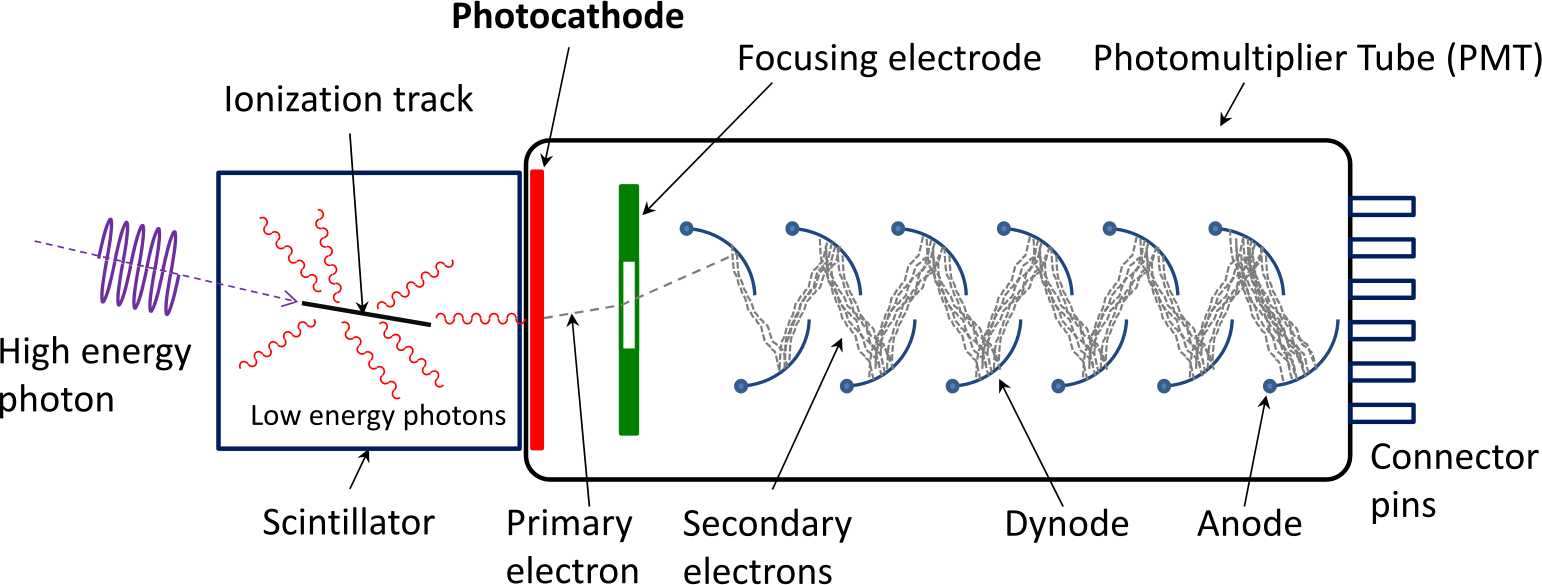
\includegraphics[width=0.9\linewidth]{Scintillator.png}
   \caption{Scintillator with PMT~\cite{wikiScin}}%
\end{figure}

\paragraph{Fast-slow coincidence} is the technique to measure the ionizing radiation separately. The "slow" part will determine the energy of incoming radiation. And the "fast" part is used to measure the time as precisely as possible, since the photomultiplier will be brought to saturation and the height of the pulse is not proportional to radiation energy any more. \textcolor{blue}{How exactly configure the fast and slow part? By adjusting the voltage?}

\paragraph{SCA} stands for single channel analyzer

\paragraph{CFD} stands for constant fraction discriminator
